% !TEX root = ../presentation.tex

\begin{frame}{Результаты работы сети}
\begin{figure}
\centering
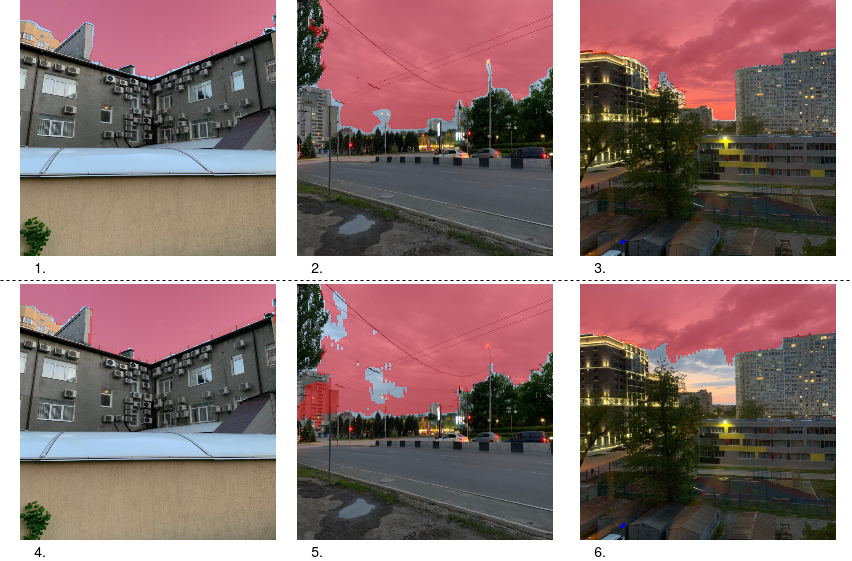
\includegraphics[width=8.52cm, height=5.61cm]{data_count_compare.png}
\end{figure}
    Верхняя тройка изображений получены с помощью сети, обученной на совмещенном датасете.
    Нижняя - сетью, в обучении которой использовался только SkyFinder.
%\textbf{$C$}-центр камеры (оптический центр); \textbf{$Cp$}-главная ось камеры
\end{frame}